%%
%% Meta: Master Document
%% Kompendium GESO
%%

%% So kann die Größe für alle Skripts direkt verändert werden
\documentclass[twoside,14pt,a5paper]{extarticle}

\usepackage{bbw}

\renewcommand{\author}{Philipp G. Freimann, nach Susanne Wagner und Urs Vonesch}
\renewcommand{\grafikautor}{Ph. G. Freimann}
\renewcommand{\authoremail}{philipp.freimann@bbw.ch}
\renewcommand{\erstellungsdatum}{19. Juli 2019}
\renewcommand{\docversion}{0.0.1 (\LaTeX{})}

\renewcommand{\doctitel}{Kompendium Mathematik}
\renewcommand{\untertitel}{Fachbereich Gesundheit / Soziale Arbeit}
\renewcommand{\fachthema}{Aufgaben}
\renewcommand{\rechte}{\textbf{Nutzungsrechte} Creative Commons CC-NB-CY}

%%%%%%%%%%%%%%%%%%%%%%%%%%%%%%%%%%%%%%%%%%%%%%%%%%%%%%%%%%%%%%%%%%%
%%%%%%%%%%%%%% A r i t h m e t i k   u n d   A l g e b r a  I
\begin{document}

\ptitlepage

%%\newpage
\newpage
\part{Repetitionsaufgaben}
%%
%% 2019 07 04 Ph. G. Freimann
%%


\section{Grundlagen Arithmetik und Algebra}

\textbf{Kompendium}\footnote{Auszug aus dem Original-``Kompendium
  Mathematik'' \cite{kompendium18} von Susanne Wagner und Urs Vonesch. Rückmeldungen und Inputs zu dieser Kopie an \texttt{philipp.freimann@bbw.ch}}

Erlaubt ist ein Taschenrechner \textbf{ohne} Computeralgebrasystem
(CAS).


\subsection{Grundlagen}
Benennen Sie die folgenden Terme mit dem richtigen Begriff
(Jeweils einer aus: \textit{Summe}, \textit{Differenz}, \textit{Produkt},
\textit{Quotient}, \textit{Potenz}):


\begin{multicols}{3}
\begin{enumerate}[label=\alph*)]
 \item $(3+x)\cdot{}2 + y$ \TRAINER{Summe}
 \item $(4a)^x$ \TRAINER{Potenz}
 \item$4a^x$ \TRAINER{Produkt}
 \item$(x-2y^4z)^2$ \TRAINER{Potenz}
 \item$2a^7 - 4bc(z-1)^3$ \TRAINER{Differenz}
 \item$(2a -b) : x + z : 4$ \TRAINER{Summe}
 \item$(a-4)(z+3)$ \TRAINER{Produkt}
 \item$(2a-b):(x+z:4)$ \TRAINER{Quotient}
\end{enumerate}
\end{multicols}

\subsubsection{Zahlmengen und zugehörige Grundoperationen}
Ordnen Sie die folgenden Zahlen der am weitesten links stehenden
Zahlmenge zu:

$$\mathbb{N} \subset \mathbb{Z} \subset \mathbb{Q} \subset \mathbb{R}$$

\begin{multicols}{2}
\begin{enumerate}[label=\alph*)]
 \item$-\sqrt{\frac{16}{2}}$ \TRAINER{$\mathbb{R}$}
 \item$|-\pi|$ \TRAINER{$\mathbb{R}$}
 \item$1.\overline{25}$ \TRAINER{$\mathbb{Q}$}
 \item$\frac{\sqrt{8}}{\sqrt{2}}$ \TRAINER{$\mathbb{N}$}
\end{enumerate}
\end{multicols}


\subsubsection{Ordnungsrelationen}
Setzen Sie zwischen die Terme (an die Stelle der drei Punkte) die
richtigen Relationszeichen ($<$, $=$, $>$):

\begin{multicols}{2}
\begin{enumerate}[label=\alph*)]
 \item$|5-2| ... |2-5|$ \TRAINER{$=$}
 \item$-\sqrt{3} ... -\sqrt{2}$ \TRAINER{$<$}
 \item$-3 ... |-3|$ \TRAINER{$<$}
 \item$\frac{1}{3} ... \frac{1}{4}$ \TRAINER{$>$}
 \item$\frac{2}{3} ... \frac{3}{4}$ \TRAINER{$<$}
 \item$2.\overline{9}$ ... 3\TRAINER{$=$}
 \item$-\frac{1}{3} ... -\frac{1}{4}$ \TRAINER{$<$}
\end{enumerate}
\end{multicols}


\subsubsection{Absolutbetrag}
Lösen Sie in der Grundmenge $\mathbb{Z}$:

\begin{multicols}{2}
\begin{enumerate}[label=\alph*)]
 \item$|x+4| = 5$ \TRAINER{$\mathbb{L}=\{1,-9\}$}
 \item$|2x-1| = 0$ \TRAINER{$\mathbb{L}=\{0.5\}$}
 \item$|-x + 7| = 10$ \TRAINER{$\mathbb{L}=\{-3, 17\}$}
 \item$|-x|=-1$ \TRAINER{$\mathbb{L}=\{\}$}
\end{enumerate}
\end{multicols}

\subsubsection{Runden}\index{Runden!Aufgaben}
Runden Sie auf 2 Dezimalen (Nachkommastellen):

\begin{multicols}{3}
\begin{enumerate}[label=\alph*)]
 \item$2.245$ \TRAINER{2.25}
 \item$2.995$ \TRAINER{3.00}
 \item$\sqrt{3}$ \TRAINER{1.73}
\end{enumerate}
\end{multicols}

Runden Sie auf vier signifikante Stellen:

\begin{multicols}{2}
\begin{enumerate}[label=\alph*)]
 \item 12.05649  \TRAINER{12.06}
 \item 0.028249 \TRAINER{0.02825}
 \item 2\,468\,900  \TRAINER{2\,469\,000}
 \item 1\,370.5   \TRAINER{1\,371}
\end{enumerate}
\end{multicols}

Runden Sie auf 2 Dezimalstellen in der wissenschaftlichen Notation:
\begin{multicols}{2}
\begin{enumerate}[label=\alph*)]
 \item 12.05649  \TRAINER{1.21 $\cdot 10^1$}
 \item 0.028249 \TRAINER{2.82 $\cdot 10^{-2}$}
 \item 2\,468\,900  \TRAINER{2.47 $\cdot 10^{6}$}
\end{enumerate}
\end{multicols}


%%%%%%%%%%%%%%%%%%%%%%%%%%%%%%%%%%%%%%%%%%%%%%%%%%
%% Summenzeichen
\subsection{Grundoperationen mit algebraischen Termen}
Schreiben Sie die Summanden hin und berechnen Sie den Wert des Ausdrucks:
\begin{enumerate}[label=\alph*)]
 \item $$\sum_{k=2}^{k=4}{(3k+2^k)}$$ \TRAINER{(6+4) + (9+8) + (12+16) = 10+17+28=55}
 \item $$\sum_{i=4}^{i=7}(3i) + 6$$   \TRAINER{((12) + (15) + (18) +(21) )+6=72}
\end{enumerate}


Schreiben Sie als Summen:

\begin{multicols}{2}
\begin{enumerate}[label=\alph*)]
\item $\left(5m-\frac{1}{2}n\right)^2$
\item $(t-9s^2)\cdot(t+9s^2)$
  \item $(3a + b^4)^2$
  \end{enumerate}
\end{multicols}

Faktorzerlegung mit Hilfe der Binomischen Formeln\index{Binomische
  Formeln!Aufgaben}

\begin{multicols}{2}
\begin{enumerate}[label=\alph*)]
\item $4x^2-y^2$
\item $36a^2 + 36ab + 9b^2$
\item $4x^4-28x^2y+49y^2$
\item $a^3-a$
\item $x^3-6x^2y+9xy^2$
  \item $z^4 -3^2$
\end{enumerate}
\end{multicols}

Faktorzerlegung durch planmäßiges Probieren

\begin{multicols}{2}
\begin{enumerate}[label=\alph*)]
\item $a^2 + 2a -15$
\item $a^3-a^2-6a$
\item $a^2 - 20a + 75$
  \item $a^2 -19a + 48$
\end{enumerate}
\end{multicols}

Faktorzerlegung durch teilweises Ausklammern und Ausklammern von
Klammern (Zerlegen Sie in möglichst viele Faktoren):

\begin{multicols}{2}
\begin{enumerate}[label=\alph*)]
\item $ab(x-2y)-b(x-2y)$
\item $x(y-2z)-(y-2z)$
\item $(a-2b)(m+n)+(a-2b)(3m+n)$
\item $3a-6ab+c-2bc$
  \item $ac-ad+bc-bd$
\end{enumerate}
\end{multicols}

Bruchterme umformen

\begin{multicols}{2}
\begin{enumerate}[label=\alph*)]
\item $\frac{st-3t^2}{s^2-st} + \frac{3s^2-3st-st+t^2}{s^2-2st+t^2}$
\item $\frac{\frac{a^2-16c^2}{8a^2}}{\frac{a-4c}{4a}}$
\item $\left(\frac{1}{a^2} - \frac{1}{b^2}\right) \cdot
    \left(\frac{a}{a+b} + \frac{b}{a-b}\right)$
\item $\left( \frac{a+4}{a} - \frac{b+4}{b}\right) : \frac{a-b}{a}$
    
\end{enumerate}
\end{multicols}


\subsection{Potenzen}

Schreiben Sie als Bruch ohne negative Exponenten:

\begin{multicols}{2}
\begin{enumerate}[label=\alph*)]
\item $2x^{-3}$
  \item $ab^{-5}$
\end{enumerate}
\end{multicols}

Schreiben Sie folgende Bruchzahlen als Dreierpotenzen:

\begin{multicols}{2}
\begin{enumerate}[label=\alph*)]
  \item $\frac{1}{9}$
  \item $\frac{1}{27}$
    \item $\frac{1}{81}$
\end{enumerate}
\end{multicols}

Lösen Sie die Exponentialgleichungen durch Erzeugen gleicher Basis:

\begin{multicols}{3}
\begin{enumerate}[label=\alph*)]
\item $2^x=\frac{1}{8}$
\item $2^{2x}=\frac{1}{8}$
\item $4^x=\frac{1}{32}$
\item $3^x=\frac{1}{81}$
  \item $9^x=\frac{1}{3}$
  \item $27^{2x}=\frac{1}{9}$
  \item $\left(3^x\right)^6 = \frac{1}{81}$
    \item $50\cdot 5^{n-1} + 3\cdot 5^{n+1} = 5^x$
    \item $\frac{25^k}{125^3} = 5^x$
      \item $2^x=\frac{8^4}{4^8}$
\end{enumerate}
\end{multicols}


Wenden Sie die Potenzgesetze an und schreiben Sie so einfach wie
möglich:
\begin{multicols}{3}
\begin{enumerate}[label=\alph*)]
\item $a\cdot a^{2x+3} : a^{1-x}$
\item $\left(\frac{x}{y}\right)^7 : \left(\frac{-x}{y}\right)^3$
\item $(-b)^6 \cdot (-b^8)$
\item $(-x^3)^4$
\item $\left( -(a^{-1})^{-2} \right)^6$
\item $(-a)^4 : (-a^{10})$
  \item $4^k \cdot \left( \frac{1}{2} \right)^k \cdot \left(
    \frac{1}{3} \right)^{-k}$
\end{enumerate}
\end{multicols}


Vereinfachen Sie:
$$\left(\frac{3x^{-2}y^2}{4x^{-4}y^3}\right)^{-2} : \left(\frac{2x^{-1}}{3xy^{-2}}\right)^3$$


Vereinfachen Sie folgende Terme. Resultat in Wurzelschreibweise:

\begin{multicols}{2}
\begin{enumerate}[label=\alph*)]
\item $\left(\frac{1}{a}\right)^{-\frac{1}{4}}$
\item $\sqrt{x}\cdot \sqrt[3]{x^4} \cdot \sqrt[6]{x^3}$
  \item $3a\cdot \sqrt[3]{9a^2}$
\item $\sqrt[4]{b\cdot \sqrt[3]{b^2\cdot \sqrt{b}}}$
\end{enumerate}
\end{multicols}

%%%%%%%%%%%%%%%%%%%%%%%%%%%%%%%%%%%%%%%%%%%%%%%%%%%%%%%%% 
\subsection{Zehnerlogarithmen}

Berechnen Sie die Exponenten. Resultate exakt, wenn nötig mit Hilfe von
Zehnerlogarithmen:

\begin{multicols}{2}
\begin{enumerate}[label=\alph*)]
\item $a^x=b$
\item $4^x=12$
  \item $4\cdot 3^{x+1}=6$
\end{enumerate}
\end{multicols}x

%%
%% 2019 07 04 Ph. G. Freimann
%%


\textbf{Kompendium}\footnote{Auszug aus dem Original-``Kompendium
  Mathematik'' \cite{kompendium18} von Susanne Wagner und Urs Vonesch. Rückmeldungen und Inputs zu dieser Kopie an \texttt{philipp.freimann@bbw.ch}}

Erlaubt ist ein Taschenrechner \textbf{ohne} Computeralgebrasystem
(CAS).


\section{Gleichungen und Gleichungssysteme}
\subsection{Lineare Gleichungen}

\subsubsection{Erfüllbare und unerfüllbare lineare Gleichungen}

Bestimmen Sie die Lösungsmenge bezüglich der Grundmenge
$G=\mathbb{R}$:

\begin{enumerate}[label=\alph*)]
\item $4x=7+3x$
\item $3x=x$
\item $(x+2)^2 + (x+3)^2 - (x+5)^2 = (x-2)^2 - 12$
\item $6x + 5 = \frac{1}{3} (18x + 15)$
\item $8x -2 = 4x + 1 - (-4x - 3.5)$
\item $\frac{3x-1}{4} + \frac{2x+1}{5} - 1 = \frac{3x-1}{5} +6 - \frac{x+2}{3}$
\end{enumerate}

\subsubsection{Lineare Bruchgleichungen (Definitions- und
  Lösungsmenge)}

Nennen Sie die Definitionsmenge, lösen Sie anschließend die Gleichung
und bestimmen Sie die Lösungsmenge; $G=\mathbb{R}$. Exakte Werte
angeben:

\begin{multicols}{2}
\begin{enumerate}[label=\alph*)]
\item $\frac{4a+6}{2a-10} + \frac{6a-43}{5-a} = -10$
\item $\frac{22.5}{a-3} + \frac{9}{-a^2 + 6a - 9} = 0$
\item $\frac{1}{x(x-4)} + \frac{1}{x(x+4)} = \frac{2}{x^2-16}$
\item $\frac{3.6x+8.5}{x^2-x-12} + \frac{5.2}{x-4} = \frac{1.9}{-x-3}$
\item $\frac{21}{-x+7} = 3 + \frac{1.5x}{\left(\frac{7-x}{2}\right)}$    
\end{enumerate}
\end{multicols}

\subsubsection{Lineare Gleichungen mit Parametern}

Bestimmen Sie die Lösungen. Schreiben Sie die Ergebnisse so einfach
wie möglich. Die Lösungsvariable ist jeweils $x$:

\begin{enumerate}[label=\alph*)]
\item $(t+x-s)(t-x-s) = (t-x)(s+x) - st$
\item $\frac{k-bx}{v} + x = \frac{vx-b}{v}$
\item $(k-4)x = 4k - k^2$
\item $\frac{1}{x} + \frac{1}{a} = \frac{1}{b}$
  \item $\frac{x- \frac{n^2}{4}}{\frac{1}{2} - \frac{n}{4}} = x+n$

\end{enumerate}

\subsubsection{Textaufgaben, die auf lineare Gleichungen führen}

\begin{enumerate}
\item
  Zerlegen Sie die Zahl 188 so in zwei Summanden, dass der 3. Teil des
  ersten Summanden um 12 kleiner ist als der 5. Teil des zweiten
  Summanden. Wie heißen die beiden Summanden?

\item Urs addiert zu einer gedachte Zahl $x$ die Zahl 5, setzt recht
  an die Summe die Ziffer 7, dividiert die entstandene Zahl durch 11,
  multipliziert den Quotienten mit 4 und erhält das 14-fache der
  ursprünglichen Zahl. Um welche Zahl $x$ handelt es sich?

\item Jemand muss zwei Kredite von zusammen CHF 180\,000.- zu 4.5\%
  und 5.5\% verzinsen. Wären die Zinssätze vertauscht, so ergäbe sich
  ein um CHF 225.- niedriger Jahreszins. Wie hoch sind die Kredite?

\item Jemand macht per 1. Juni eine Einlage von CHF 75\,000.- bei
  einem Zinsfuß von 3.5\%. Einige Monate später erhöht sich der
  Zinsfuß um 1.5\%, so dass am Jahresende auch ein um CHF 281.25
  höherer Zins als ursprünglich erwartet resultiert. Wann fand die
  Erhöhung statt?

\item Eine Buchhandlung verkaufte von den vorhandenen Exemplaren eines
  neu erschienen Krimis am ersten Tag ein Achtel und 10 Stück, am
  zweiten Tag vom Restbestand die Hälfte und 15 Stück. Danach blieben
  noch 50 Krimis übrig. Wie viele Exemplare waren ursprünglich
  vorhanden?

\item Ein Kaufmann mischt 6\,kg einer Warensorte mit 14\,kg einer
  zweiten Sorte. Der Preis je kg der ersten Sorte ist um CHF 2.50
  höher als derjenige der zweiten Sorte. Er erhält eine Mischung, die
  CHF 8.- pro kg kostet. Wie teuer ist jede der beiden Sorten pro kg?

\item Aus 60\%-igem und 65\%-igem Alkohol sollen 150 Liter 63\%-ige
  Mischung hergestellt werden. Wie viele Liter von jeder Sorte muss
  man verwenden?

\item Auf dem Flohmarkt wird um ein Ölbild gefeilscht. Der Händler
  verlangt CHF 590.-, während der Käufer nur CHF 410.- bezahlen
  will. Die beiden einigen sich so, dass der Händler den Preis um
  gleich viele Prozente senkt, wie der Käufer sein Angebot
  erhöht. Welches ist der Verkaufspreis und um wie viele Prozente sind
  beide von ihren Forderungen abgewichen?

\item Wenn zwei Zuleitungen gleichzeitig geöffnet sind, füllen sie ein
  Bassin in 9 Minuten und 36 Sekunden. Um das Bassin alleine zu
  füllen, braucht die erste Zuleitung 12 Minuten. Wie lange benötigt
  die zweite Zuleitung, wenn sie das Bassin alleine füllen soll?

\item Eine Weinhändlerin kauft 300 Liter Rotwein und 600 Liter
  Weißwein. Der Preis pro Liter Weißwein ist um CHF 1.50 höher als der
  Literpreis Rotwein. Weil der Weinbauer und die Händlerin alte
  Freunde aus der BM-Schulzeit sind, erhält die Weinhändlerin pro
  Liter Rotwein 10\% und pro Liter Weißwein 12\% Rabatt.
  Der Weinbauer vertauscht jedoch die beiden Rabatte und schickt der
  Händlerin somit eine Rechnung, die um CHF 60.- zu hoch ist.
  Berechnen Sie die Literpreise für Rot- bzw. Weißwein vor Abzug der
  Rabattes.
\end{enumerate}


\subsection{Gleichungssysteme mit zwei Unbekannten}

  Bringen Sie die Gleichungen auf die Grundform und lösen diese
  anschließend mit dem Taschenrechnermodus.

  Bestimmen Sie die Lösungsmenge bezüglich der Grundmenge $G = \{(x,
  y) \in \mathbb{R}\times\mathbb{R}\}$;

\begin{multicols}{2}
  \begin{enumerate}
  \item
    
    \gleichungZZ{-\frac{x}{2}}{2y-1+x}{\frac{x}{2}+3}{1-x}

  \item
    \gleichungZZ{\frac{a+b}{6}}{\frac{a}{2}-5}{a+8}{\frac{b+a}{6}}

  \item
  \gleichungZZ{5x-8y}{1}{20x}{7+32y}

\item
  $$2x+7y = -5+8y = 24x +7$$
\item
  \gleichungZZ{3x}{2+5y}{6}{\frac{24}{3x} + \frac{10y}{x}}

\item
  \gleichungZZ{\frac{4x-1}{5}-x}{y-\frac{3y-4}{2}}{\frac{x+y-3}{2x-y+7}}{\frac{3}{4}}
  
  \end{enumerate}
\end{multicols}


  \subsection{Substitution (zwei Gleichungen, zwei Unbekannte)}

\begin{multicols}{2}
  \begin{enumerate}
  \item
    \gleichungZZ{\frac{b}{a+b}}{1-\frac{3}{a-b}}{\frac{3b}{a+b}}{1-\frac{2}{a-b}}

  \item
    \gleichungZZ{\frac{2y}{4x-1}+9}{\frac{5}{x+2y}}{\frac{10}{x+2y}-12}{\frac{y}{4x-1}}
  \end{enumerate}
\end{multicols}

  \subsection{Textaufgaben}

  \begin{enumerate}
  \item
    Farben der Sorte A und der Sorte B mit Kilopreisen von CHF 12.-
    bzw. CHF 10.- werden gemischt. Ein Kilogramm Mischung kommt nun
    auf CHF 10.90 zu stehen. Nähme man bei gleicher Gesamtmenge der
    Mischen von der Sorte A 3 kg weniger, so würde das Kilogramm nur
    noch CHF 10.40 kosten. Wie viele kg nahm man anfänglich von jeder
    Sorte?

    \item Frau Groß hat ein Kapital in zwei Posten angelegt, einen zu
      4\% und einen zu 5\%. Nach ihrer Rechnung beträgt die Summe der
      Jahreszinsen CHF 2\,560. Das sind aber CHF 80.- zu viel; sie hat
      nämlich die Zinssätze verwechselt. Welche Posten hat sie zu
      welchem Zinssatz angelegt?

      \item Dividiert man eine zweiziffrige Zahl durch ihre Quersumme,
        so erhält man 4 Rest 9. Vertauscht man die Ziffern der
        ursprünglichen Zahl und dividiert diese durch die um 13
        vermehrte Quersumme, so erhält man 3.


        \item Eine Händlerin kaufte 800 Stück von Sorte I und 400
          Stück von Sorte II für insgesamt CHF 4\,200. Sorte I
          verkaufte sie mit einem Zuschlag von 15\% und Sorte II mit
          einem Zuschlag von 50\%. Der Verkaufspreis betrug insgesamt
          CHF 5\,180. Für wie viel Geld hatte sie ein Stück jeder
          Sorte eingekauft?
          
    \end{enumerate}


  \subsection{graphisches Lösen von linearen Gleichungssystemen}

  \begin{enumerate}
  \item Lösen Sie das Gleichungssystem grafisch für
    $-20 \leq x \leq 80$ und $-50 \leq y \leq 100$.

    \gleichungZZ{10y}{7.5x}{18.75x+25y}{1500}

    \item Lösen Sie das Gleichungssystem grafisch für
      $-10 \leq x \leq 10$ und $-10 \leq y \leq 10$.

      \gleichungZZ{3x+y-9.5}{4y-\frac{28}{7}}{-\frac{4}{5}y + x}{-5+0.2x}

          \item Lösen Sie das Gleichungssystem grafisch für
      $-50 \leq x \leq 50$ und $-50 \leq y \leq 50$.

            \gleichungZZ{40}{-2y-x}{3.5x -5y +82}{4\left(x-y+\frac{51}{2}\right)}

  \end{enumerate}


  \subsection{Quadratische Gleichungen}

  Lösen Sie die Gleichungen ohne Solve-Funktion des Taschenrechners,
  indem Sie sie auf die Grundform bringe. Die Grundform kann
  anschließend mit dem entsprechenden Taschenrechnermodus gelöst
  werden.

  \subsubsection{Reinquadratische Gleichungen}
  Bestimmen sie $x$:
  \begin{multicols}{2}
  \begin{enumerate}
  \item $x^2 = 0.04$
  \item $x^2+4=0$
  \item $(7+x)(7-x)=(3x+2)^2-(2x+3)^2$
    \item $\frac{x-3}{x+3} + \frac{x+3}{x-3} = \frac{26}{x^2-9}$
  \end{enumerate}
  \end{multicols}

  \subsubsection{Gemischtquadratische Gleichungen: Lösungsformel}
  Grundform:

  \begin{tabular}{|c|c|}%%
    \hline%%
Grundform: $ax^2 + bx +c = 0$ & Lösungsformel: $x_{1,2} = \frac{-b \pm \sqrt{b^2 - 4ac}}{2a}$\\%%
    \hline%%
    \end{tabular}%%

  Bestimmen Sie $x$:
  \begin{multicols}{3}
  \begin{enumerate}
  \item $0 = 12x^2 - 8x - \frac{4}{3}$
  \item $3x^2 + 5x = -1$
  \item $-5x^2 = 20 + 7.5x$
  \item $\frac{1}{8}x^2 + 2.5x + 8 = 0$
  \item $\frac{x-4}{x-5} = \frac{30-x^2}{x^2-5x}$
    \item $\frac{x}{3} - \frac{x^2-19}{3x+6} = 3 + \frac{4x-7}{6-3x}$
    \end{enumerate}
    \end{multicols}

  \subsubsection{Quadratische Gleichungen: Substitution}
  Gleichungen höheren Grades, die durch Substitution auf eine
  quadratische Gleichung führen:

  \begin{enumerate}
  \item Lösen Sie die Gleichung nach $x$ auf. Resultate exakt:
    $$\left(x-\frac{3}{x}\right)^2 - 20 = x - \frac{3}{x}$$

  \item Lösen Sie die Gleichung nach $x$ auf und runden Sie das
    Resultat auf drei Dezimalstellen:
    $$(x+7)^6 = 8\cdot (x+7)^3 - 15$$

  \item $$(x+7)^8 = 14(x+7)^4 + 32$$
  \end{enumerate}


    \subsection{Textaufgaben, die auf quadratische Gleichungen führen}
Die Gleichungen sind auf Grundform zu bringen und können anschließend
mit dem entsprechenden Taschenrechnermodus gelöst werden.

\begin{enumerate}
  \item Ein Speicher wird durch eine Zuleitung in einer bestimmten
    Zeit gefüllt. Das Entleeren durch eine andere Leitung dauert eine
    Minute länger. Aus Unachtsamkeit bleibt während des Füllens die
    andere Leitung geöffnet, deshalb ist der Speicher erst nach 756
    Minuten voll. Wie lange dauert die Leerung des Speichers bei
    geschlossener Zuleitung?

    \item Das Produkt der beiden kleinsten von sechs aufeinander
      folgenden natürlichen Zahlen ist dreimal so groß wie die Summe
      der vier übrigen Zahlen. Wie heißt die kleinste Zahl?

      \item Eine Praxiseinrichtung mit einem Anschaffungswert von CHF
        24\,000;.- wurde zweimal mit dem gleichen Prozentsatz
        abgeschrieben und hat zur Zeit einen Wert von CHF 16\,335.-.
        Wie viele Prozente beträgt der Abschreibungssatz?

      \item Dividiert man die Summe zweier positiver Zahlen durch ihre
        Differenz, so erhält man 12.5\% der größeren Zahl.
        Berechnen Sie die größere Zahl, wenn die kleinere 42 ist.

        \item Die Zehnerziffer einer zweiziffrigen Zahl ist um 6
          kleiner als die Einerziffer. Die vierfache Summe der
          Quadrate der Ziffern ist gleich der fünfunzwanzigfachen
          Quersumme. Wie heißt die Zahl?
\end{enumerate}


\subsection{Elementare Potenzgleichungen mit ganzzahligen und
  rationalen Exponenten}
Lösen Sie die Gleichung ohne Solve-Funktion des Taschenrechners nach
$x$ auf und schreiben Sie die Resultate als exakte Werte ($G =
\mathbb{R}$):

\begin{multicols}{3}
\begin{enumerate}
\item $\frac{2}{3}x^3 = 12$
\item $x^5 = \frac{1}{32}$
\item $\left(\frac{1}{x}\right)^6 = 13$
\item $\left(\frac{x-5}{3}\right)^3=64$
\item $(x+5)^{\frac{1}{2} = 4}$
\item $\left(x-6\right)^{\frac{1}{3}} = 2$
\end{enumerate}
\end{multicols}


  \subsection{Elementare Exponentialgleichungen}
Lösen Sie die Gleichung ohne Solve-Funktion des Taschenrechners nach
$x$ auf und schreiben Sie die Resultate als exakte Werte ($G =
\mathbb{R}$).
Tipp: Erzeugen gleicher Basis

\begin{multicols}{3}
\begin{enumerate}
\item $2^x=16$
\item $\left(\frac{1}{4}\right)^x = 64$
\item $2^x\cdot 8^{x-1} = 32$
  \item $\left(\frac{1}{3}\right)^x\cdot \left(\frac{3}{27}\right)^x = 3$
  \item $e^{2x}=1$
  \item $\frac{6^{x-2}}{36^{x+1}} = 216$
  \item $\left(3^x\right)^6=\frac{1}{81}$
    \item $2^x + 2^{x+3} = \frac{9}{4}$
  \end{enumerate}
\end{multicols}

%%
%% 2019 07 04 Ph. G. Freimann
%%


%%%%%%%%%%%%%%%%%%% 4. Datenanalyse %%%%%%%%%%%%%%%%%%%%%

\section{Datenanalyse}

\textbf{Kompendium}\footnote{Auszug aus dem Original-``Kompendium
  Mathematik'' \cite{kompendium18} von Susanne Wagner und Urs Vonesch. Rückmeldungen und Inputs zu dieser Kopie an \texttt{philipp.freimann@bbw.ch}}

Erlaubt ist ein Taschenrechner \textbf{ohne} Computeralgebrasystem
(CAS).


\subsection{Vorbemerkungen}
\paragraph{Abkürzungen}

$n$ = Anzahl Werte

$Q_1$ = erstes Quartil

$IQR$ = Interquartilsrange = Quartilsdifferenz = $Q_3 - Q_1$

$\varsigma$ = Standardabweichung (Nenner $n$).

$\overline{x}$ = empirischer Mittelwert

$med$ = Median

$Q_3$ = drittes Quartil

$R$ = Range = Spannweite

\paragraph{Zur Berechnung der empirischen Standardabweichung}
Frommenwiler \cite{frommenwiler17alg} verwendet den Nenner $n$
(Stichprobenvarianz). Es sollen bei der Korrektur beide Varianten:
Nenner = $n$ bzw. Nenner = $n-1$ akzeptiert werden, da eine vertiefte
Einsicht erst in der schließenden Statistik der Fachhochschule
vermittelt wird.

\paragraph{Zur Berechnung der Quartile}
In Literatur und Statistikprogrammen existieren verschiedene Methoden
der Quartilsberechnung.

\subsection{Grundlagen}

\begin{enumerate}
\item Das Säulendiagramm zeigt die Anzahl Kinder pro Familie in einer Siedlung mit
$n=150$ Familien (10 Familien haben keine Kinder, 25 Familien haben 1
  Kind, ...).

\makebox{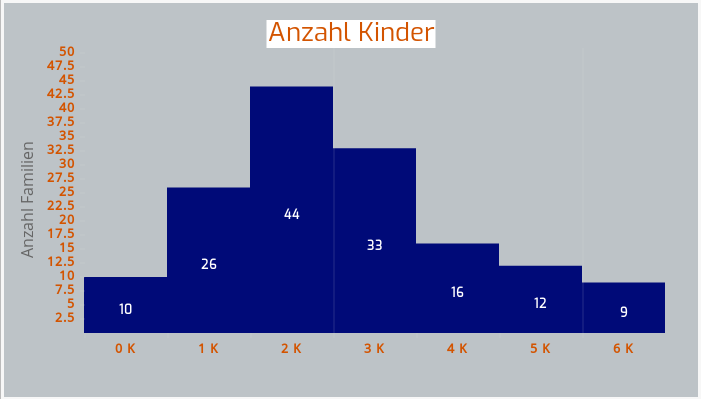
\includegraphics[width=10cm]{img/statistic_anz_familien_anz_kinder.png}}

a) Berechnen Sie die relativen Häufigkeiten als Dezimalzahl (3
Dezimalen) und in Prozenten (1 Dezimale).

b) Berechnen Sie die durchschnittliche Kinderzahl pro Familie

c) Erklären Sie anhand dieses Beispiels die Begriffe

\textit{Stichprobenumfang\index{Stichprobe}\index{Stichprobenumfang}, Merkmalsträger\index{Merkmalsträger}, Merkmal\index{Merkmal}, Merkmalsprägung\index{Merkmalsprägung},
  absolute Häufigkeit\index{absolute
    Häufigkeit}\index{Häufigkeit!absolute}, relative
  Häufigkeit\index{relative Häufigkeit}\index{Häufigkeit!relative}}

d) Wie viele Kinder leben in dieser Siedlung?

\item

  Gegeben sind folgende Rohdaten:

  7, 5, 3, 8, 1, 2, 10, 5, 8, 9, 2

  \begin{enumerate}[label=\alph*)]
  \item Erstellen Sie eine geordnete Liste.
  \item Auf welchem Rang\index{Rang} befindet sich der Wert 3?
    \item Welcher Wert befindet sich auf dem mittleren Rang?
  \end{enumerate}

  \subsubsection{}

  
\end{enumerate}


\subsection{Datenerhebung: Problematik von Ausreißern}

\begin{enumerate}
\item Das Durchschnittsvermögen in einer kleinen Gemeine mit 250
  steuerpflichtigen Personen betrug CHF 175\,600.-.

  Durch den Zuzug einer einzigen vermögenden Person erhöhte sich
  dieser Durchschnitt auf CHF 220\,900.-. Wie hoch ist das Vermögen
  dieser Person?

\item Das monatliche Durchschnittseinkommen in einer Firma mit 850
  Beschäftigten beträgt CHF 7\,250.-. Die drei Spitzenverdiener dieser
  Firma verdienen monatlich je CHF 86\,000.-.
  Berechnen Sie das monatliche Durchschnittseinkommen, wenn diese drei
  Spitzenwerte nicht berücksichtigt werden.

\item
  In einer Schulklasse ergaben sich bei der Auswertung einer Prüfung
  folgende Punktezahlen:

  35, 58, 59, 4, 38, 43, 45, 52, 49, 55

  a) Berechnen Sie Mittelwert und Median.

  b) Berechnen sie den Mittelwert ohne den Ausreißer 4.

\item
  10 Eier haben folgende Gewichte in Gramm:

  52.8, 55.9, 58.2, 57.1, 60.4, 69.1 57.9, 58.0, 62.5, 65.0

  Nun wird aus Jux zu den Eiern ein Gips-Ei hinzugelegt. Dadurch
  erhöht sich das Durchschnittsgewicht um 3.48 Gramm pro Ei.

  Berechnen Sie das Gewicht des Gips-Eies.

  Runden Sie auf 0.1 Gramm genau.
  
\end{enumerate}


\subsection{Diagramme (Säulendiagramm, Histogramm, Boxplot)}

\begin{enumerate}
\item \textbf{Säulendiagramm}

  In einer Ausstellung wurden im Laufe einer Woche folgende
  Besucherzahlen ermittelt:

  \begin{tabular}{lllllll}
    Montag & Dienstag & Mittwoch & Donnerstag & Freitag & Samstag & Sonntag \\
    350    & 321      & 647      & 519        & 844     & 1\,314  & 2\,522
  \end{tabular}

  Zeichnen Sie ein \textbf{Säulendiagramm} mit den relativen
  Häufigkeiten in \%.

\item \textbf{Säulendiagramm und Boxplot}

  Hier sehen Sie die Prüfungspunkte in einer Klasse.

  1) Urliste:

  76, 74, 82, 96, 66, 76, 78, 72, 52, 86, 84, 76, 78, 92, 82, 74, 88,
  62

  2) Hier sehen Sie die selben Zahlen geordnet:

  52, 62, 66, 72, 74, 74, 76, 76, 76, 78, 78, 82, 82, 84, 86, 88, 92, 96

  \begin{enumerate}[label=\alph*)]
  \item
    Teilen Sie die Daten in Klassen ein: [50; 60), [60; 70), usw.
        \textit{(Klassenbreite = 10 Punkte).} Zeichnen Sie ein
        Säulendiagramm mit den relativen Häufigkeiten. Zeichnen Sie
        die Säulen aneinanderstoßend.

      \item
        Zeichnen Sie einen \textbf{Boxplot}.
      \item
        Bestimmen Sie den \textbf{Mittelwert}.
      \item
        Bestimmen sie den \textbf{Modalwert} (Modus).
      \item
        Bestimmen Sie die \textbf{Quartilsdifferenz} \textit{IQR}.
    \end{enumerate}

\item \textbf{Klassendiagramm, Säulendiagramm, Boxplot}
 Die Messung der Körpergröße von 100 18-jährigen Schülern liefert
 folgende Zahlen:

 \begin{tabular}{lcccccccccc}
   Größe in cm & 163 & 164 & 165 & 166 & 167 & 168 & 169 & 170 & 171 & 172\\
   Anzahl      &  1  &  1  &  1  &  3  &  3  &  3  &  4  &  6  &  5  &  5
   \end{tabular}

 \begin{tabular}{lcccccccccc}
   Größe in cm & 173 & 174 & 175 & 176 & 177 & 178 & 179 & 180 & 181 & 182\\
   Anzahl      &  4  &  7  &  6  &  5  &  5  &  7  &  5  &  4  &  4  &  6
   \end{tabular}

  \begin{tabular}{lcccccc}
   Größe in cm & 183 & 184 & 185 & 186 & 187 & 188\\
   Anzahl      &  5  &  3  &  3  &  2  &  1  &  1 
  \end{tabular}

  \begin{enumerate}[label=\alph*)]
  \item Erstellen Sie eine Klasseneinteilung mit Klassenbreite 5cm:

    Klasse 1: [160cm; 165cm)

      Klasse 2: [165cm; 170cm)

        usw.

        Zeichnen Sie anschließend ein Säulendiagramm mit den relativen
        Häufigkeiten in Prozent. Zeichnen Sie die Säulen
        aneinanderstoßend.

        \item Zeichnen Sie einen Boxplot mit diesen Daten.
\end{enumerate}


\item \textbf{Vergleich zweier Boxplots}

  Wurfweiten beim Ballwurf in Metern:

  Versuchsreihe 1:

  34.0, 34.4, 32.2, 33.5, 35.2, 32.9, 32.6, 34.3, 33.2, 34.1,
  33.2, 33.2, 34.0, 32.7. 34.8, 33.5, 33.5

  Versuchsreihe 2:

  32.8, 33.7, 34,9, 34.3, 34.6, 32.3, 34.0, 33.9, 33.0, 32.4,
  31.1, 35.5, 31.7, 34.8, 33.5, 32.4

  Erstellen Sie für beide Versuchsreihen je einen Boxplot (Darstellung
  mit gleicher Skala, sodass ein Vergleich möglich wird).



  \item{Informationen aus einem Diagramm herauslesen}

    Praliné-Kugeln in einer Packung; Darstellung der absoluten
    Häufigkeiten:
    
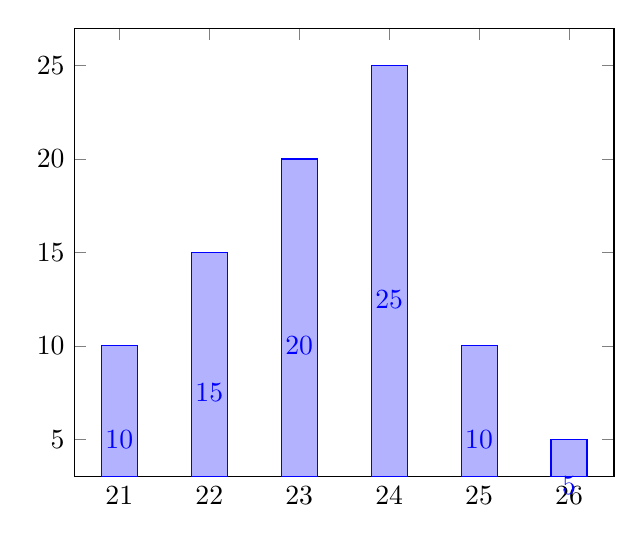
\begin{tikzpicture}\begin{axis}[ybar stacked,nodes near coords,bar
      width=0.4,]\addplot
    coordinates{(21,10) (22,15) (23, 20) (24, 25) (25, 10) (26, 5)};\end{axis}\end{tikzpicture}

Bestimmen Sie Mittelwert, Median und Standardabweichung.
Rechnen Sie mit den Klassenmitteln.

\end{enumerate}


\subsection{Maßzahlen (Mittelwert, Media, Quartile,
  Standardabweichung, Quartilsdifferenz)}

\textit{Einige Lehrplanziele dieses Kapitels wurden bereits in den
  vorhergehenden Aufgaben behandelt: Geordnete Liste, Klassenbildung,
  Mittelwert (mit Ausreißer-Problematik), Median, Standardabweichung,
  Quartilsdifferenz.}

\begin{enumerate}
\item In einer Klasse wurden folgende 18 Prüfungsnoten erzielt:

  \begin{tabular}{llllllllll}
    3 & 3 & 3.5 & 3.5 & 4   & 4 & 4.5 & 4.5 & 4.5 & 4.5\\
    5 & 5 & 5.5 & 5.5 & 5.5 & 6 & 6   & 6
  \end{tabular}

  Berechnen Sie \textbf{Mittelwert} und \textbf{Standardabweichung}
  mit Hilfe des Rechners.

\item Drei \textbf{Streumaße}: \textbf{Spannweite R (Range)},
  \textbf{Quartilsdifferenz IQR}, \textbf{Standardabweichung $\sigma$}

  Gegeben sind folgende Daten, die bereits geordnet sind:

  \begin{tabular}{llllllllll}
    2.5 & 2.8 & 3.2 & 3.5 & 3.5 & 4.1 & 4.2 & 4.7 & 4.8 & 4.8\\
    5.4 & 5.5 & 6
  \end{tabular}

  Ermitteln Sie die \textbf{Spannweite (Range)}, die
  \textbf{Quartilsdifferenz} und die \textbf{Standardabweichung} (auf
  2 Dezimalen genau).
  
  
  \end{enumerate}


%%%%%%%%%%%%%%%%%%%%%%%%%%%%%%%%%%%%%%%%%%%%%%%%%%%%%%%%%%%%%%%%%%%
%%\newpage\mbox{}
%%\blankOddPage{}%
%\include{texlife-bibtex-extra}
 \bibliography{bibAll}{}\label{literatur}

 \printindex
%%%%%%%%%%%%%%%%%%%%%%%%%%%%%%%%%%%%%%%%%%%%%%%%%%%%%%%%%%%%%%%%%%%

\end{document}
